\section{Theory}

\subsection{How does Augmented Reality work?}
There are different types of augmented reality. Some of those are marker-based, location-based, superimposition-based and projection-based. \\

\textbf{Marker-based} AR is when markers, in the form of images have to be placed in the real world and detected by the application. Virtual object are rendered on top of these markers. An example would be a picture in a magazine which, when pointing a camera at it, the application renders an 3D object on top.\\

\begin{figure}[hbtp]
\begin{center}
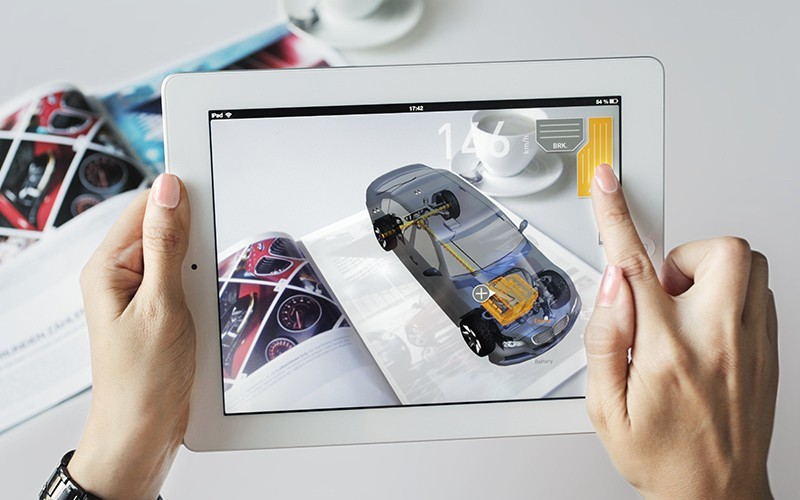
\includegraphics[width = 0.75\textwidth]{./Images/markerbasedar.jpg} 
\caption{A virtual object in the form of a car being rendered on top of a marker in a magazine.}
\end{center}
\end{figure}

\textbf{Location-based} AR is when the content on the users screen differs depending on the location of the user. This type is highly dependent on the GPS signal.
An example of where this could be useful is in a museum where different information could be given to the user depending on which room he is in.\\

\textbf{Superimposition-based} AR uses object recognition in order to enhance that object with some sort of visual information. It replaces the real object with an enhanced virtual one. It could be used in retail to display different patterns on a piece of clothing.\\

\textbf{Projection-based} AR is when virtual object can be placed in a room to make it appear as if they were there. A popular example of this would be the IKEA Place app that was mentioned in the introduction.  \\

\begin{figure}[hbtp]
\begin{center}
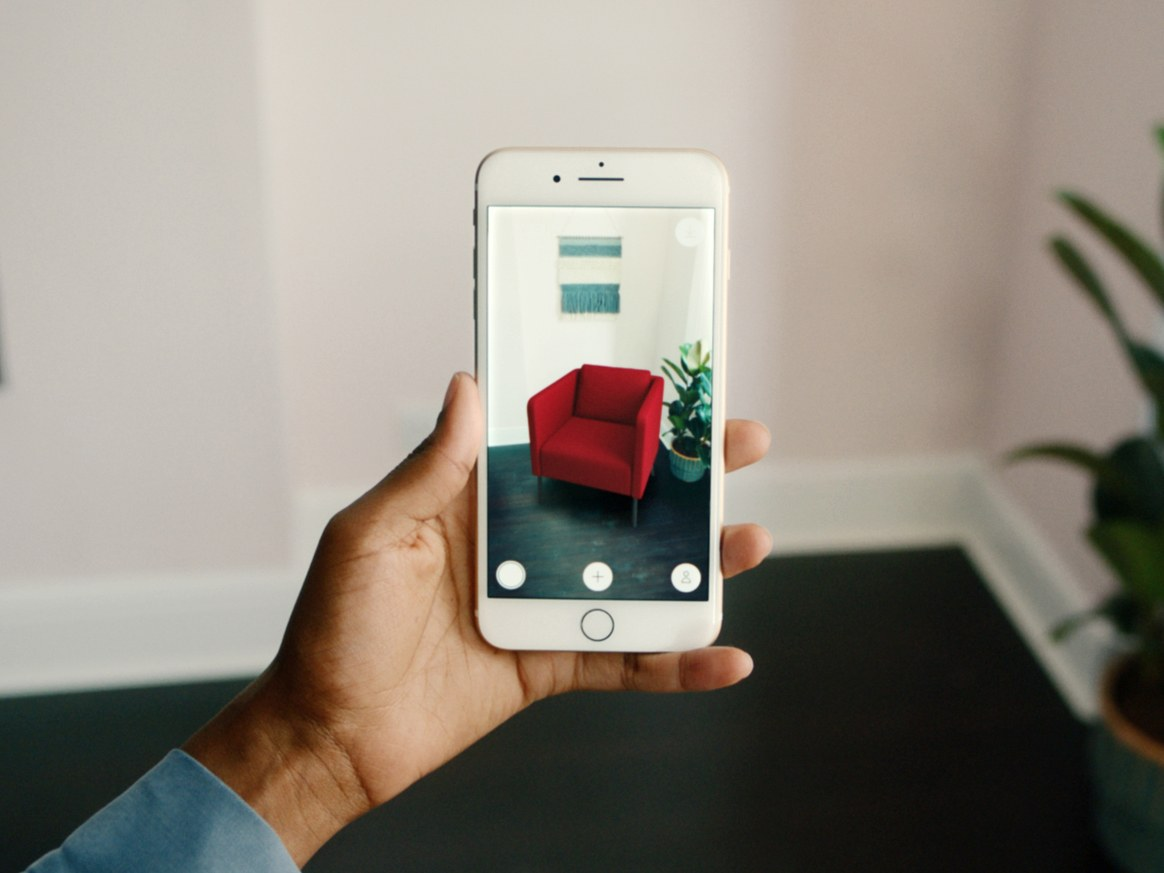
\includegraphics[width = 0.75\textwidth]{./Images/ikeaplace.jpg} 
\caption{A virtual sofa chair being added to a room within the IKEA Place app.}
\end{center}
\end{figure}

In this paper we will mainly be using projection based AR with a form of recognition. The projections will be in the form of way-pointers used as instructions for the user to perform the next step in putting together a furniture piece. These instructions can visualize how the pieces will look like after the step is completed, and to show arrow pointers between the pieces that are supposed to be put together.

\subsubsection{History of AR}
The idea of augmented reality has existed a long time, the phrase has only been used for about 28 years but it is not until recently that the technology has become mainstream.
This is mainly due to it becoming good enough to be used by the average person at home. Today we can just download an app on our smart phones to enjoy the technology. Below follows a brief history of how augmented reality has progressed throughout the years.\\

\textbf{1968}
The Sword of Damocles - The first mounted headset.
This device was mounted on the head and could display a cube wireframe floating in the air. It was invented by Ivan Sutherland.\\

\textbf{1975}
Myron Krueger - Videoplace. Using cameras to interact with a digital world with shadows.
This application could be used to draw things or play simple video games with the shadow of your hand.
\cite{videoplace}\\

\textbf{1990}
The first time the term "Augmented Reality" was used by the Boeing researcher Tom Caudell.\\

\textbf{2009}
AR comes to the web in the form of an open source toolkit called ARToolKit.\\

\textbf{2017}
Apple launches AR Kit and Google launches AR Core.\\

\subsubsection{S.L.A.M.}
S.L.A.M (Simultaneous Localization and Mapping) is a way for a machine to get to know the environment that it is in. It registers features and maps them to its surroundings. S.L.A.M is about having the map of the environment and knowing where the robot is in that map.
The problem with this is that a map is needed for knowing where you are, and you have to know where you are to be able to create a map. That is why S.L.A.M is doing this at the same time, hence 'Simultaneous'. The system is used in autonomous robots, but also valuable in Augmented Reality. \cite{slam}

iPhone X does this by tracking multiple reference points in space and from them building a 3D model of the surroundings using a form of S.L.A.M technique.
This is accomplished by keeping a map of the features while keeping track of the path the observer is taking. A number of 
hardware components make this task possible, including gyro, accelerometer and a compass. \cite{iphoneslam}

\begin{figure}[hbtp]
\begin{center}
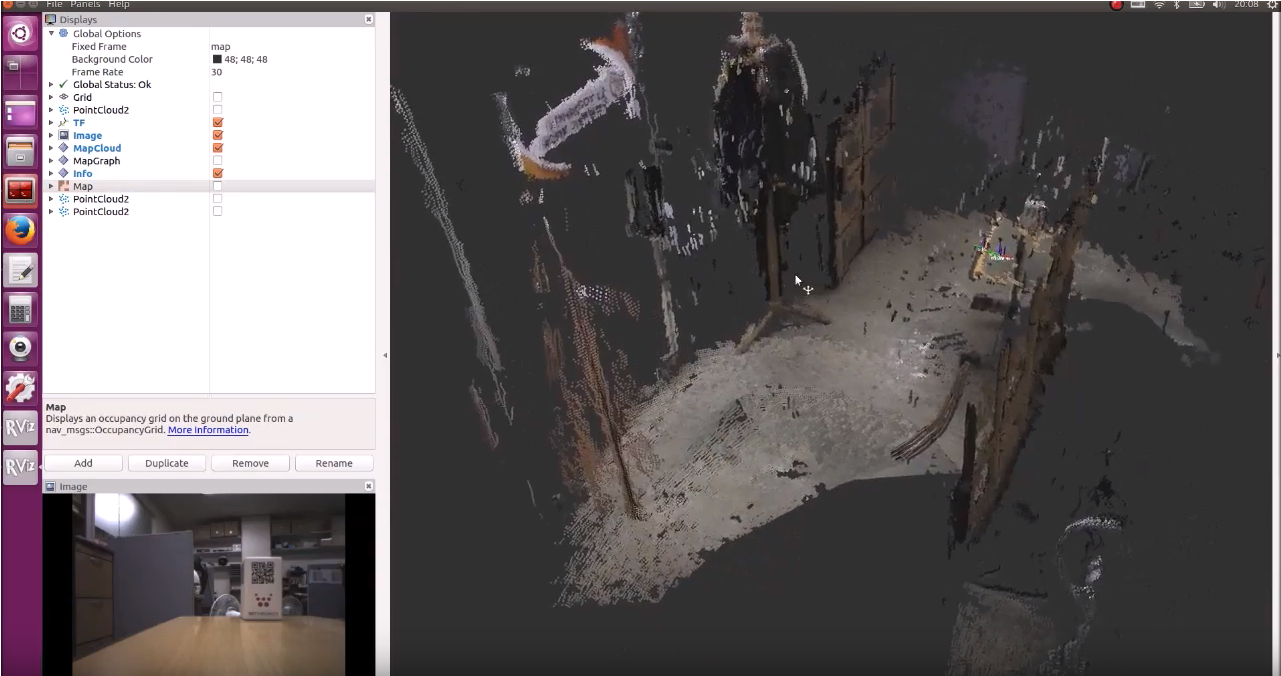
\includegraphics[width = 0.75\textwidth]{./Images/slam-map.jpg} 
\caption{A robot performing S.L.A.M in an environment and the 3D model created.}
\end{center}
\end{figure}

\subsubsection{Other inputs}
Compass, Gyroscope, Accelerometer  etc.

\subsubsection{How does ARKit work?}
ARKit works similar to SceneKit were a scene (which is basically a 3D environment in which nodes containing 3D models (geometry) can be rendered) is loaded at start up and interacted with.
An ARScene is contained inside an ARSCNView (AR Scene View) which also has a ARSession
that that manages the motion tracking and camera image processing. For an ARScene to work, it must have a running ARSession.
The session is started with configuration (ARConfiguration). This configuration can be of many kinds, the most common ones begin ARWorldTrackingConfiguration and ARFaceTrackingConfigurations. For this project, ARWorldTrackingConfiguration will be used since the face tracking one uses the front camera.

Below, an example of how to setup a configuration and running a session is given:

\begin{lstlisting}[language=swift]
func loadWorldTrackingConfiguration()
    {
        let configuration = ARWorldTrackingConfiguration()
        configuration.planeDetection = [.horizontal]

        // All the objects that are tracked is contained in the Objects folder
        guard let detectingObjects = ARReferenceObject.referenceObjects(inGroupNamed: "Objects", bundle: nil) else { return }
        configuration.detectionObjects = detectingObjects
        
        // Setting up tracking of images
        for imageURL in trackingImageURLs
        {
            guard let image: CGImage = UIImage(named: imageURL)?.cgImage else { return }
            let referenceImage = ARReferenceImage(image, orientation: CGImagePropertyOrientation.up, physicalWidth: 0.3)
            configuration.detectionImages.insert(referenceImage)
        }

        configuration.maximumNumberOfTrackedImages = trackingImageURLs.count
        
        sceneView.session.run(configuration)
    }
\end{lstlisting}

But before a session can be started, an ARScene must exists and be loaded. The ARScene is a regular .scn file that has the starting nodes that together form the starting
environment the user will interact with. An example of how a scene like that looks like is shown in figure \ref{fig:3dsceneImage}.

\begin{figure}[hbtp]
\begin{center}
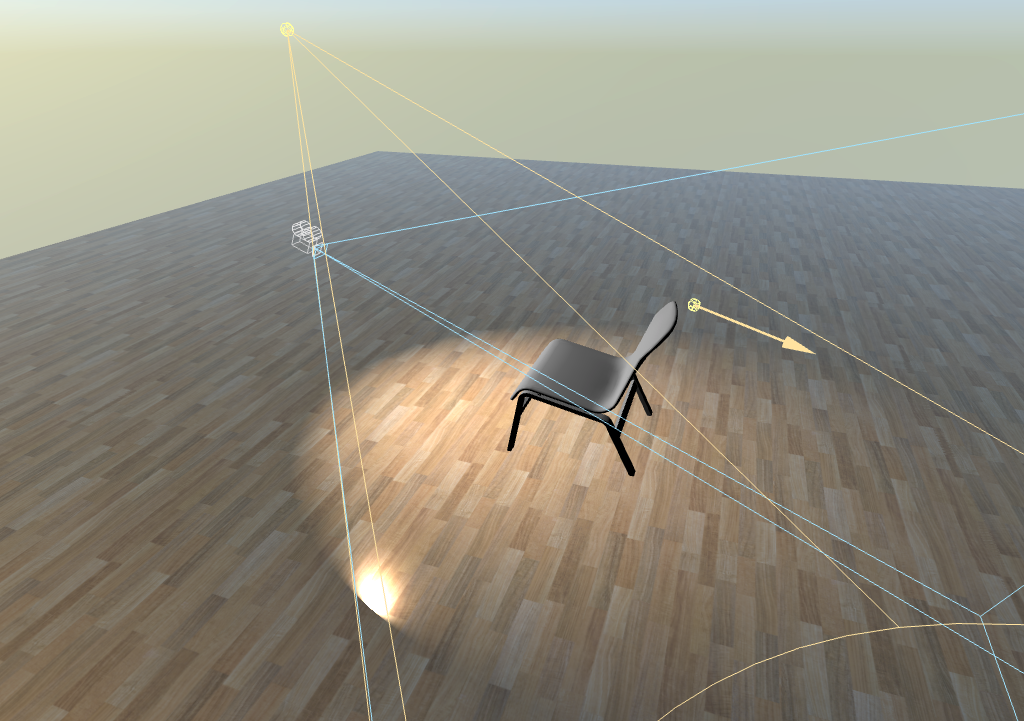
\includegraphics[width = 0.75\textwidth]{./Images/3dscene.jpg} 
\caption{An example of a 3D scene created in XCode with a camera, a plane, directional light and three geometry nodes.}
\label{fig:3dsceneImage}
\end{center}
\end{figure}

To load a scene, a new .scn file must be created in the art.scnassets folder and fetched like below.
\begin{lstlisting}[language=swift]
// Load the scene
let scene = SCNScene(named: "art.scnassets/world.scn")!        
sceneView.scene = scene
\end{lstlisting}

When ARScene detects objects, images, planes etc. it calls the renderer function. This function can be implemented by setting the ViewController to conform to the ARSCNViewDelegate. ARScene adds an anchor (ARAnchor) and a node (SCNNode) for the place where it detected it, and this can be used inside the function to render new nodes or other logic.

\begin{lstlisting}[language=swift]
func renderer(_ renderer: SCNSceneRenderer, didAdd node: SCNNode, for anchor: ARAnchor)
    {
    	    // If detected an object
        if let objectAnchor = anchor as? ARObjectAnchor
        {
            let objectName = objectAnchor.referenceObject.name!
            let textNode = GeometryFactory.makeText(text: objectName)
            node.addChildNode(textNode)
        }
        // If detected a plane
        else if let planeAnchor = anchor as? ARPlaneAnchor
        {
            node.addChildNode(GeometryFactory.createPlane(planeAnchor: planeAnchor, metalDevice: metalDevice!))
            model.numberOfPlanesDetected += 1
        }
    }
\end{lstlisting}

If nodes need to be rendered outside of this function it can be done by accessing the
scenes root node.

\begin{lstlisting}[language=swift]
sceneView.scene.rootNode.addChildNode(node)
\end{lstlisting}

\subsection{What Machine Learning methods are there?}
There exists many different machine learning techniques out there today. Due to its high effectiveness and relevance, for this report we are going to focus on the highly popular method of artificial neural networks.
This is a proven method for working well with images (Convolutional neural networks) and is therefore a highly 
relevant technique for this project.

\subsubsection{Perceptron}
A perceptron is the simplest form of the neural network. It has a set of inputs and an output.
The perceptron first sums up all the input values, x, multiplied with the weight value, w.
After that it passes that sum through an activation function. This activation function can be everything from a simple f(x)=x to the more complex sigmoid function, depending on the need. More on this in the upcoming section.

\begin{figure}[hbtp]
\begin{center}
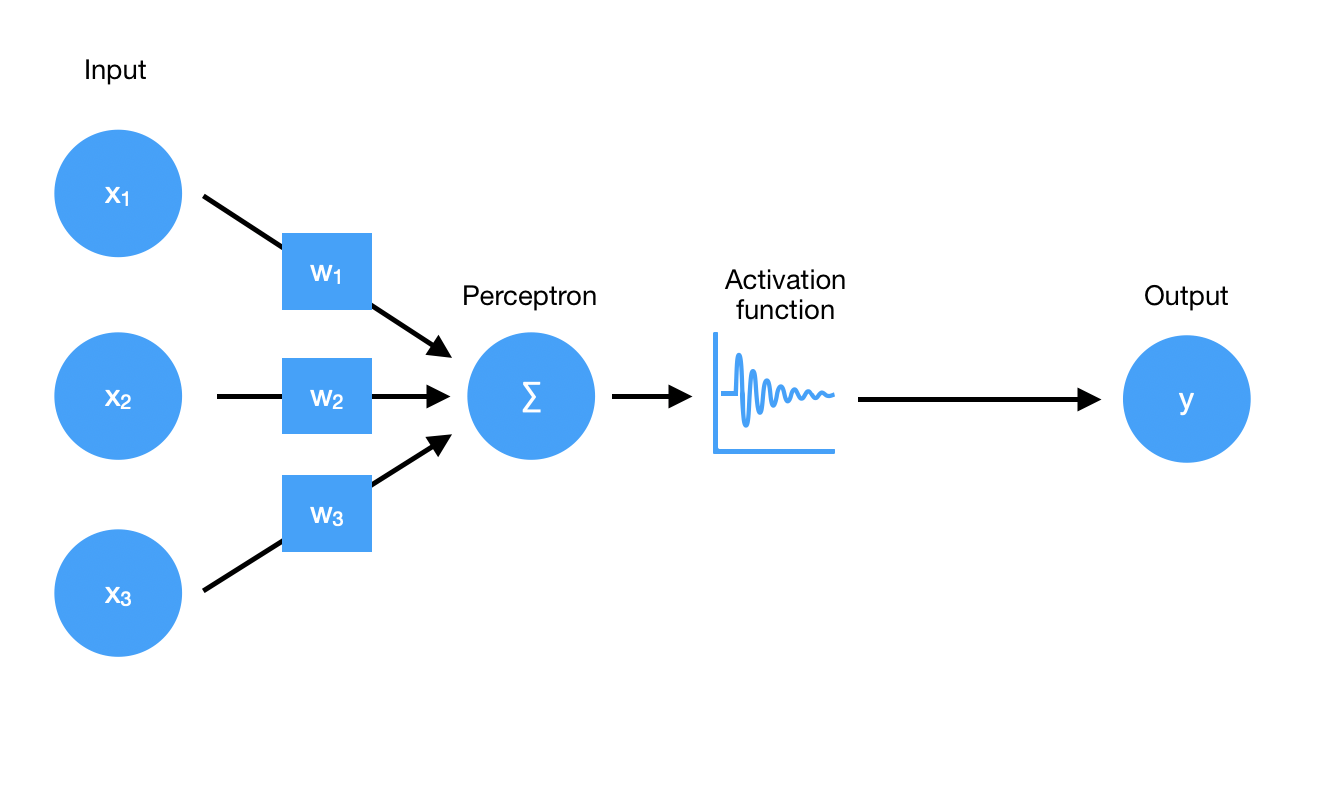
\includegraphics[width = 0.75\textwidth]{./Images/perceptron.jpg} 
\caption{An illustration of the perceptron, the simplest version of a neural network.}
\end{center}
\end{figure}

A bias also exists in every node which is not based on any input. The bias function in the perceptron is similar to what the m in $y = kx + m$ does. It gives the function the ability to move up and down in the graph for more possibilities of splitting the data set. The bias is usually disregarded when illustrating the perceptron.

The perceptron only has the ability to draw a single line and thus is only able to split simple data sets.

The output of the perceptron is described by the following formula:

\[ y = b + \displaystyle\sum_{i=1}^{n} x_i \cdot w_i \]

where b is the bias value, x is the input, w is the weight for that input and n is the number of inputs.

\subsubsection{Activation functions}

The activation function,  $ \phi (v_{i}) $ , takes the sum of all the inputs from a node as input and passes them through a function before giving an output. This is beneficial when for instance the output should be kept in a range between 0 and 1, or perhaps when negative values don't make sense.
Usually, activation functions are attributed to layers instead of individual nodes.

The most common of these functions are \textbf{ReLu}, \textbf{Tanh}, \textbf{Sigmoid} and \textbf{Softmax}.

\textbf{ReLu} is described as
\[f(x) = max(0, x)\]
and is a good option when negative values should be ignored or don't make sense. Problems with ReLu?

\textbf{Tanh} is the tangens hyperbolicus function and is used to output values either as -1 or 1 like a binary operator. Unlke a binary operator, tanh's derivative is always defined which makes back propagation possible.

\textbf{Sigmoid} is described as 
\[\frac{e^x}{1+e^x}\]
and works like the Tanh function but keeps the values between 0 and 1 and sets y(0) = 0.5 instead.

\textbf{Softmax} is a little bit more complex. It takes a vector $v$ of dimension $n$ and turns it into a vector $\sigma(v)$ of the same dimension where $\displaystyle\sum_{i=1}^{n} \sigma_i(v) = 1 $ and each element value is between zero and one.

Each element in the array is described as below
\[ \sigma_i(v) = \frac{e^{v_i}}{\displaystyle\sum_{j=1}^{n} e^{z_k}} \]

This output is good for describing the probability for each element to be correct and is therefore commonly used
in the output layer.

\subsubsection{Calculating the loss}
When training the model, it will at first make a guess to what the right answer or value is based on the random initial weigh values. In the beginning, the model is usually mostly wrong and it is then important to know how wrong it was and in what direction it should go.

For this, the model uses a loss function to calculate that error. For different applications the loss function can be different.
One way to calculate the error is to simply take the predicted value and subtract it with the correct value, $ error = y_p - y_c $.

Sometimes the sign of the error is not important. Then the absolute error can be calculated instead. $error = |y_p - y_c| $

Another approach is the \textbf{mean squared error} which squares the difference and takes the mean value over a few predictions.
\[Error = \frac{1}{n} \cdot \displaystyle\sum_{i=1}^{n} (y_p - y_c)^{2} \]


\subsubsection{Optimizers}
Once the error has been calculated, the network will make changes to itself to improve the performance by decreasing the error value. This is called backpropagation.
The principle behind backpropagation is to go backwards in the network from the output node and determining how each weight value, $ \omega_{ik} $, should change.\\

A popular method for minimizing the error is to use \textbf{Gradient Decent} which works by ,step by step , go in the negative direction that minimize the error.
The direction is determined by taking the derivative of the error function.
The new weight value is calculated accordingly. $\eta$ is a chosen parameter called the learning rate.

\[ \Delta \omega_{ik} = -\eta \frac{\delta E}{\delta \omega_{ik}} \]

\begin{center}
where the error function is
\end{center}

\[E = \frac{1}{N} \displaystyle\sum_{i=1}^{N} E(n) \]

\begin{center}
which leads to
\end{center}

\[ \Delta\omega_{ik} = \frac{1}{N}  \displaystyle\sum_{i=1}^{N} \Delta\omega_{ik}(n) \]

The most common form of gradient decent is called \textbf{Stochastic gradient decent}.
The difference is that SGD only evaluates on a small number of nodes/patterns and updates all the weights from that observation.

\[ \Delta\omega_{ik} = \frac{1}{P}  \displaystyle\sum_{i=1}^{P} \Delta\omega_{ik}(p) \]

\textbf{Adam} (which is short for Adaptive moment estimation) is another optimizer which is quite popular.
The reason is because it has been proven to be a very effective algorithm in many different use cases.

Adam is a kind of combination of using \textbf{RMSPROP} and SGD with momentum.
Without going into too much detail, SGD with momentum keeps track of which direction the the improvement is in and keeps the improvement going in that same way. The optimisation goes faster when the previous direction is the same and slower when they are different. Almost like a rolling ball that gains speed as it is rolling down hill.
RMSPROP does something similar and uses a running average of each weight value and the previous values importance can be controlled with a parameter. It also only uses the sign of the direction and NOT its value. Also RMSPROP has individual weights.

Adam keeps a running average of both the past gradients and the squared past gradients.
The full mathematical description of Adam is given by

\[ \omega_i (t+1) = \omega_i(t) - \eta \frac{m_i}{\sqrt{v_i} + \epsilon} \]

where

\[ m_i (t+1) = \beta_1m_i(t) + (1 - \beta_1) \frac{ \delta E(t) }{\delta\omega_i} \]

\[ v_i (t+1) = \beta_2v_i(t) + (1 - \beta_2) (\frac{ \delta E(t) }{\delta\omega_i})^2 \]

and $ \eta, \beta_1 $ and $ \beta_2 $ is adjustable parameters and $ \epsilon $ a small value to keep the equation from dividing by zero.\\

There are a lot of other optimizers such as \textbf{Adagrad}, \textbf{Adadelta}, \textbf{Nadam} etc. They all have their own advantage and use-cases. We won't go into further details about them.

REFERENCE TO THE BOOK

\subsubsection{Layers}

\begin{figure}[hbtp]
\begin{center}
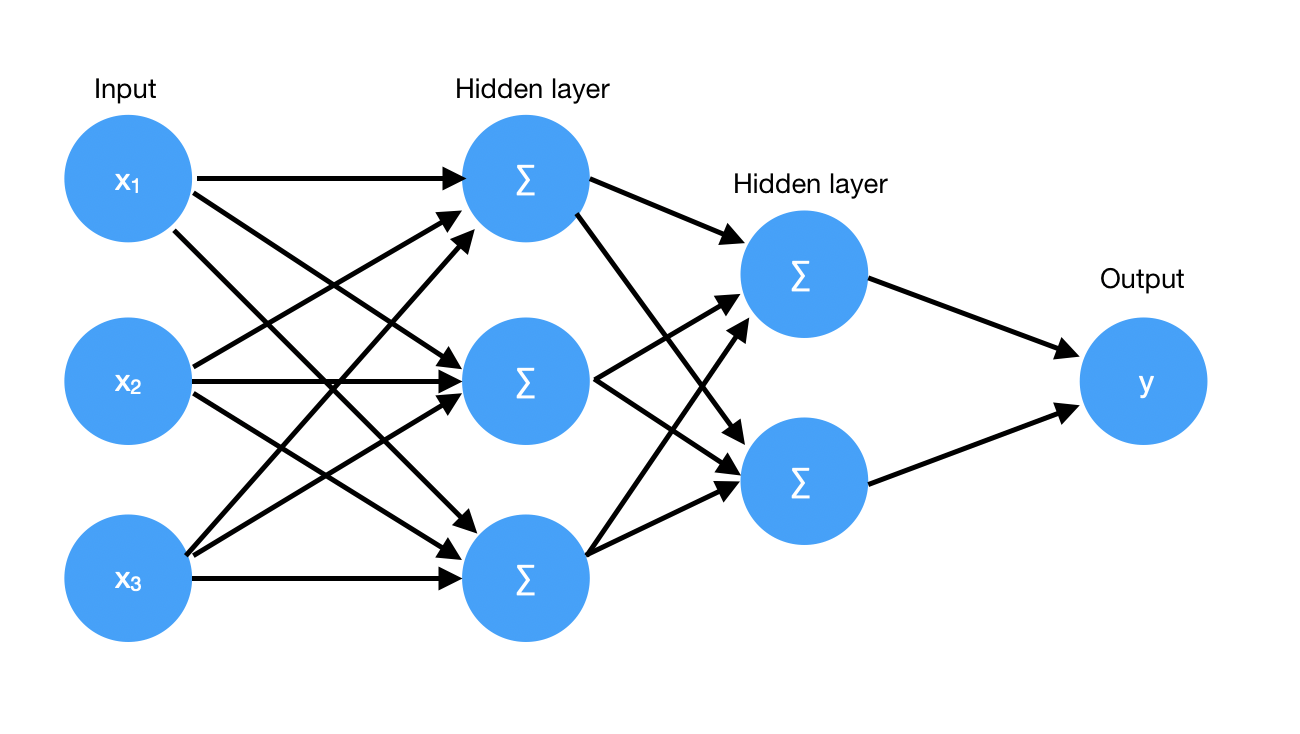
\includegraphics[width = 1.0\textwidth]{./Images/fully_connected.jpg} 
\caption{Two fully connected layers. One with 3 neurons and one with 2 neurons.}
\end{center}
\end{figure}

With more layers and more neurons the networks parameters and complexity begins to grow. So does also the training time, size of the model and the cost for doing predictions. Thus, these networks are capable of describing much more complex data sets. But as a result of that, the risk of overfitting (The act of describing the training data set too well so that new data sets will not get recognized. More on this soon.) becomes much greater. That is why a complex network is not always wanted.

\subsubsection{Overfitting}
When training a neural net, one needs to be careful not to train the model too much or overfitting is likely to happen. Overfitting is when a model gets REALLY good at predicting the data that it is training on but fails to predict accurately on new data. This is because it starts to pick up too much on detail or in some instances even noise. For this reason it fails to pick up the general trends, which is more valuable. 

\begin{figure}[hbtp]
\begin{center}
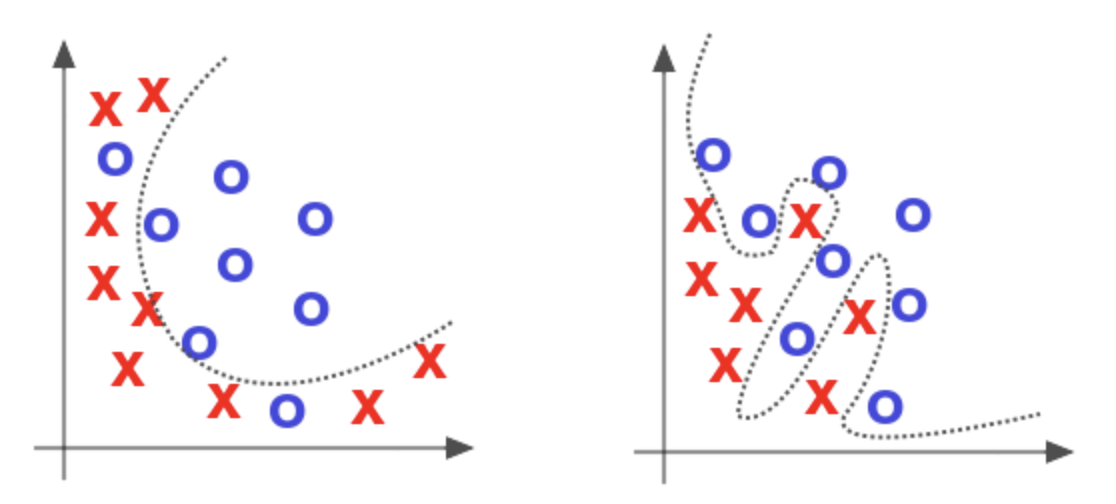
\includegraphics[width = 1.0\textwidth]{./Images/overfitting.jpg} 
\caption{Overfitting of a dataset. On the left is a accurate trained model, on the right is an overtrained model. Image taken from OReilly.com}
\end{center}
\end{figure}

\cite{overfitting}

There are tricks for combating overfitting. They usually involve trying to limit the size of a small amount of weights.
The hypothesis behind this is that if a weight is much larger than the rest it also has much more influence over the final prediction. That way, a small detail in the data can have much more influence than the general trend.

One way to do this is to cut random connections between layers during epochs, usually by specifying a certain amount that is going to be cut.
This way, the model is not relying on a small number of nodes to make the correct predictions. This method is called dropout.

Another way is to introduce random noise on a layer during training. This works because if a node with a large weight receives noise, it will be heavily amplified and probably give a false prediction.
When doing this, Gaussian noise is usually implemented, which is basically random noise with a gaussian distribution.

To force the model to keep weights small, one way is to add a penalty to the loss for every weight based on its size. 
This is called weight regularisation and is widely used and exists in two forms, L1 and L2.
L1 simply adds the weights size multiplied with an l1 term that is chosen by the designer.
The other, L2, is to do the same but in this case square that value. This has the effect of making values over 1 even bigger and values less than 1 smaller.
In that way, it doesn't affect the loss as much as L1 when not being overtrained. L2 is also called weight decay and is the more common method of the two.

Another way to keep the values between 0 and 1 is to normalize the input to every layer. In Tensorflow, this can be done with the BatchNormalization layer.

One important thing to point out is that all these methods mentioned so far are only active during training and is not doing anything when making real predictions.


If lots of training data exists, the ensemble technique could be a good way to go. This technique divides the training data into more smaller sets and trains a model for every data set.
The final prediction is then an average of the predictions of all the models. This technique works because if the model is highly overtrained in a certain direction, chances are that the other networks will drown out this result by the many other models.

It is kind of like when someone has an off pitch in a big choir. If there are many other singers, this off-pitch will not be noticed very much.

\begin{figure}[hbtp]
\begin{center}
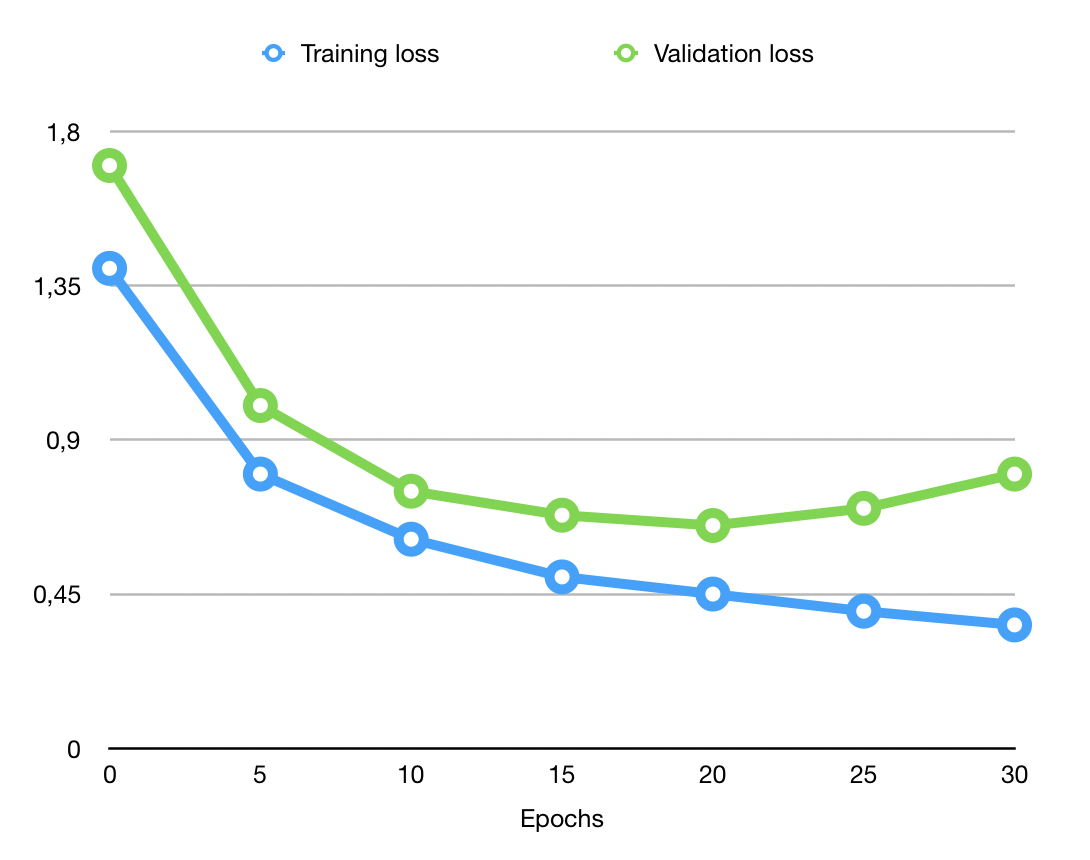
\includegraphics[width = 0.75\textwidth]{./Images/early_stop.jpg} 
\caption{A graph showing when to do an early stop. The graph shows the total loss over trained epochs. Notice that the validation starts to increase again somewhere after epoch 20.}
\end{center}
\end{figure}

The final technique is called early stopping and is based on validating the model after every epoch and stopping the training when the validation loss, or some other criteria, is not improving anymore.

\subsection{Object Detection with traditional machine learning}
% Write about feature based detection and segmentation

When trying to detect objects in a still image we have looked into two main methods. One typical way is to try and look for patterns or features in the image.
Either a specific image can be matched within the larger image or a series of features can be found.
An example of the latter is Haar features which is used in the Viola-Jones for face detection. Using the image integral (which is the summation of pixel values in a specific region) different features can be obtained.

\begin{figure}[hbtp]
\begin{center}
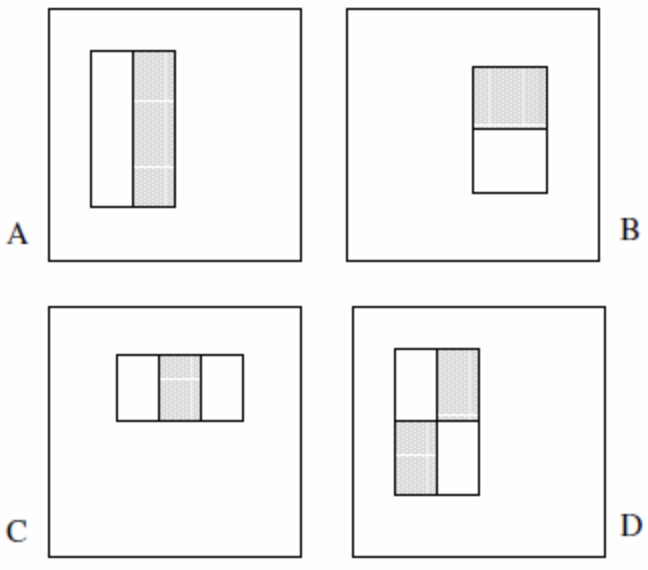
\includegraphics[width = 0.75\textwidth]{./Images/viola-jones.jpg} 
\caption{A set of Haar features used to detect faces in the Viola-Jones method. The pixels in the white regions are summed and subtracted with the pixels in the black region. The algorithm will later decide if a specific feature has been found or not, depending on obtained value.}
\end{center}
\end{figure}

This method is based on the fact that every face shares some basic similarities. Even objects of the same type can share some similarities.\cite{violaJones}
\\\\
Another way to find objects in an image is to try to classify each pixel as either background or foreground, usually referred to as Foreground/Background-segmentation. This usually requires some background knowledge of how the background usually looks like, for example, if the background is grass or a concrete floor.

One of the most basic functions for separating background and foreground is the flood fill method.
Anyone that has used Paint for Windows knows exactly what this one is. It fills a segment of similar pixels with the same color. This method works best on one backgrounds with only one color.
Online there are many different variations but they all accomplish the same goal.\cite{floodFill}
\\\\
Mathematical morphology

Edge detection

Histogram equalisation
\\\\
One possible way of detecting objects in an image is to use depth data, or RGB-D.
A tool that typically comes to mind when reading about depth data is the Kinect camera
for Xbox.

On the iPhone X, depth data can be captured by either True Depth on the front camera or with the dual cameras on the back. The True Depth camera works by having a dot projector emit light dots (mainly on a face which is why this feature is found on the front camera) and picking those dots up with an infrared camera.

The dual camera on the back works by taking two photos and comparing those to find the pixel shifts of the same objects. The distance is calculated by \[ \frac{pixelShift} { pixelFocalLength \cdot baselineInMeters}\] and gives the unit in $1/meter$. It is the same principal to how we humans see distance by having two eyes pointing the same direction. \cite{depthMap}

However, obtaining the depth data from the dual cameras in real time is not possible since it requires too much computational power. This unfortunately makes it impossible to use in an ARScene and thus not possible for this project.\\

Despite all the available methods above, object detection without machine learning is still very tricky. These methods works best when the images are in an controlled environment, typically industrial, like finding screws on a white background (as they do in an article posted by combine.se). \cite{combine}
When the environment is a more casual place tough, like recognizing furniture indoors, the task becomes much more difficult. For this reason, object detection with pure algorithms is not very common in household applications. Instead object detection with machine learning methods such as RCNN networks are much more common nowadays.

\subsection{Object Detection with deep learning}
% Write about how one can do object detection by the use of ML

Big advantages with this is that classification and detection can be done in the same
 step. For this project that is really desirable.
 
 \subsubsection{Convolutional Neural Networks}

 Convolutional neural networks have been used for quite some time when it comes to deep learning and their capabilities are rather astounding, as proved by Krizhevsky et al \cite{NIPS2012_4824}.  They use layers which perform convolutions, hence it's name.  The input to a convolutional network are either 2D or 3D tensors, where the 3D alternative usually has color channels along the third dimension. Use of convolutional neural networks in image recognition for several reasons, e.g. it can tell of spatial relationships in an image. This section has been written with reference to V. Dumolin et al \cite{convArit}. Figure \ref{fig:cnn} shows an example of how a CNN may look.
 
 \begin{figure}[hbtp]
\begin{center}
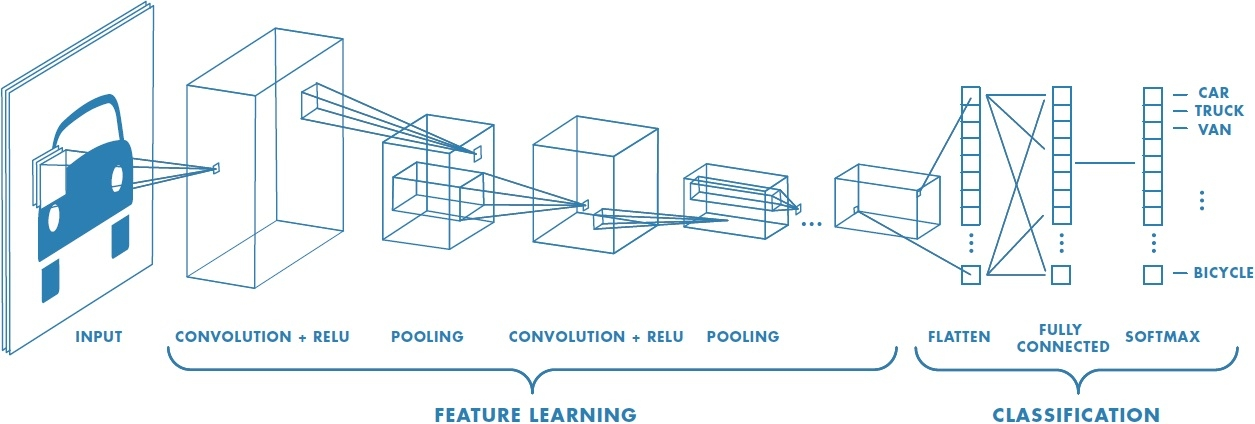
\includegraphics[width = 0.9\textwidth]{./Images/convNetwork.jpg}
\caption{Image shows the flow of a convolutional neural network from left to right. Several convolutions as well as pooling functions are done in order on the input image. The last feature map is then flattened to fit into the hidden layers, to then be classified with a softmax function. Image taken from \cite{cnnImage}}.
\label{fig:cnn}
\end{center}
\end{figure}
 
 A convolutional layer performs the mathematical operation \textit{convolution} on the input tensor, which can be presented as an image. A kernel of size $k \cdot l$ slides across the input and sums pixel values that is included inside the kernel; a new image containing these sums is the output. Padding on the input can be used to account for values when the kernel is outside the input. Use of padding have an impact on the output size after the convolutional layer. Stride is also be used, which tells how much the kernel translates along an axis;  increased stride leads to subsampling.. Since changes of parameters in one axis doesn't affect outcome in another axis it simplifies explaining CNNs by having the parameter values being the same along both axes. The more convolutional layers used in a network, more complex shapes are detected. First layers may detect edges and corners, whereas, later layers may find features representing a car or a dog. A common addition to the layers are an activation function, commonly ReLU, which has been described earlier in the report. This gives faster training by only allowing for positive weights to pass the layer.

 The common types of padding is \textit{no zero}, \textit{same} and \textit{full}; examples seen in figure \ref{fig:padding}. No Zero padding involves having no padding outside of the input. This means that the kernel never goes outside of the actual image, once a side of the kernel hits the side of the input it jump down to the next line (if stride is 1). 
 
 Same padding is used when one desires the output size of the layer to be the same as the input size. This is achieved by having a padding $p$ be $ p = \floor{\frac{k}{2}} $ for any odd kernel size $k$.
  
 With full padding one actually makes the output size larger than the input, by fully utilizing the every possible combination of the kernel and the input image. This is accomplished  by having the padding $p $ be $p = k - 1$ for any kernel size $k$. 
 
 
 \begin{figure}[hbtp]
\begin{center}
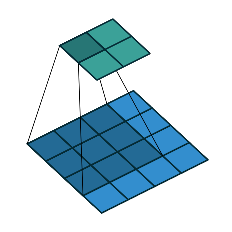
\includegraphics[width = 0.3\textwidth]{./Images/noPad.png}
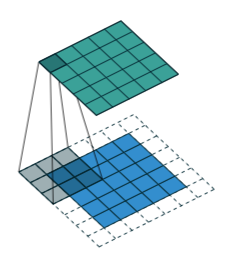
\includegraphics[width = 0.3\textwidth]{./Images/samePad.png}
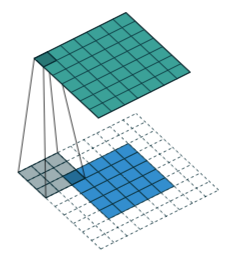
\includegraphics[width = 0.3\textwidth]{./Images/fullPad.png} 
\caption{Different examples of padding. Grid in green is the output, grid in blue is the input, and area in shadow is the current area kernel is at. Leftmost image shows a no zero padding being used. Here the kernel size is $k = 3$, input size is $i = 4$ and the output size is  $o = 2$, i.e., smaller then input.  In the middle image same padding is used; output size is the same as input size $o = i = 5$. In the rightmost image full padding is used. Here a bigger output size than the input size is produced, $o = 7, i = 5$. Images taken from \cite{convArit}}
\label{fig:padding}
\end{center}
\end{figure}
 
 
 Another useful feature used in a lot of convolutional neural networks is pooling. Pooling layers are somewhat similar to convolutional layers in that they use a sliding window which performs an operation on the contents of the window and outputs a new value. However, the difference is that they use other functions instead of linear addition. Two common pooling functions are \textit{max pooling}, where the output is the largest value within the window, and \textit{average pooling}, where the output is the average of the components within the window.  Pooling is commonly done do reduce the size of the input. Figure \ref{fig:pooling} shows example of pooling being used.
 
 \begin{figure}[hbtp]
\begin{center}
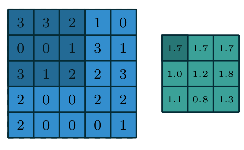
\includegraphics[width = 0.45\textwidth]{./Images/avgPool.png}
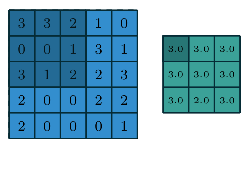
\includegraphics[width = 0.45\textwidth]{./Images/maxPool.png}
\caption{Examples of two types of pooling. Blue grid represents input, green grid represents the output, and the shaded area is where the sliding window is located. The left image shows the use of average pooling, while the right one shows the use of max pooling.
Images taken from \cite{convArit}}
\label{fig:pooling}
\end{center}
\end{figure} 
 
When a classification is to be done in the CNN, the shape needs to be shifted to an array. This is done after the last pooling layer or convolutional layer. This array can then be passed into a hidden layer for classification.

\subsubsection{RCNN and its different forms}

How to calculate loss in RCNN

Selective search for detecting regions of interest (RoI)

Fast R-CNN
" reduce the time consumption related to the high number of models necessary to analyse all region proposals."

Instead of having many CNNs for each region, one CNN is applied to the whole image.

Faster R-CNN
Segmentation is slow
Regional proposal network (RPN) is used instead

Mask R-CNN
Outside our scope, but something that can be used to improve object tracking.
Although, then an object tracking algorithm that tracks on an outline is required.

\subsubsection{YOLO}
YOLO, or You Only Look Once, is a one stage detector approach to object detection and
 recognition \cite{YOLO1}. It takes an image and predicts both bounding boxes and the probabilities of the classes being within these bounding boxes in one run, hence its name. It was designed to be fast and usable in real-time scenarios. Since YOLO sees the entire image during training and testing, it receives contextual information about the classes and reduces error with matching background patches for objects. 
 
 The architecture for \textit{YOLO} consist mainly as a convolutional neural network, with 24 convolutional layers and two fully connected layers. There was also a smaller neural network trained called \textit{Fast YOLO} trained which were only 9 layers which was designed to create an even faster system for object detection. 
 
 The system first divides the input image into an  $S \times S$  grid, where each cell predicts $B$ amount of bounding boxes respectively confidence scores for the boxes. Each bounding box prediction consist of 5 separate predictions: the \textit{x, y} coordinates, represented as their position relative to the the grid cell, width and height relative to the entire image and a confidence value. The confidence values are there to reflect how certain the model is that there exists an object within the box, i.e. ideally, confidence should be zero when no object, and the intersection over union between ground truth and the predicted box if there is. Each grid cell also predicts $C$ probabilities for each class, conditioned that there's an object within the boxes. 
 
 Intersection over union, also known as the Jaccard index, is a way of measuring similarity between sets. It can be written as 
 \[
IOU(A,B) =  \frac{|A\cap B |}{|A\cup B|} =\frac{|A\cap B|}{|A| + |B| - |A \cap B|}
, \quad 0\leq IOU(A,B) \leq 1
 \]
 if $A,B$ are two finite sets. If the two sets are equal, then \[ IOU(A,A) =  \frac{|A\cap A |}{|A\cup A|} = \frac{|A\cap A|}{|A| + |A| - |A \cap B|}  = \frac{A}{A} = 1 \]
 
 When testing, these scores are then combined to give the class specific confidence values for each of the boxes, thus it receives both the confidence of the class being in the box, and how well the box fits the object. Figure \ref{fig:YOLO_stages} summarizes the flow in YOLO. 
\begin{figure}[hbtp]
\begin{center}
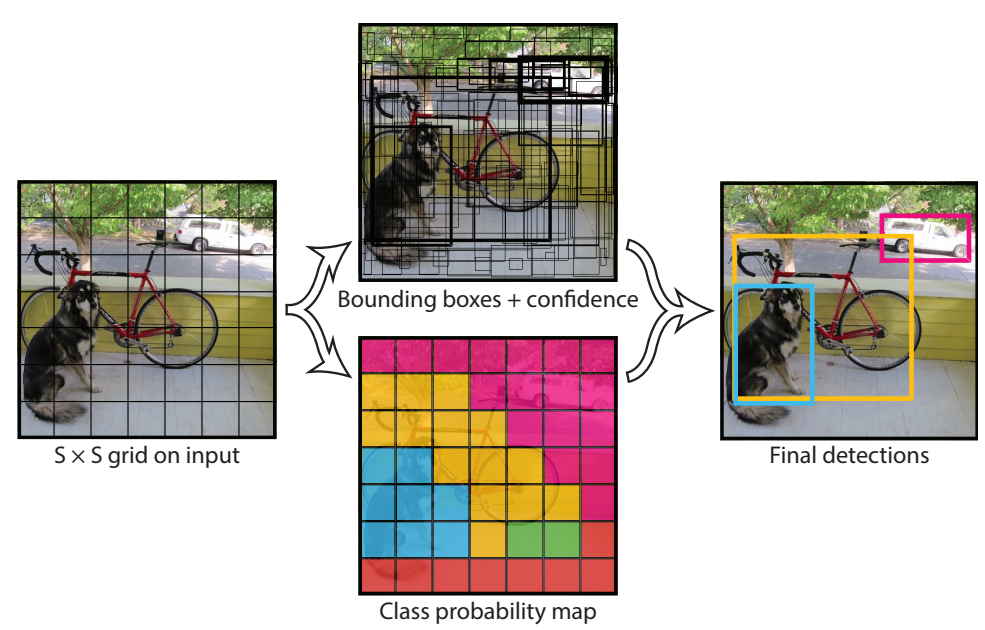
\includegraphics[width = 0.75\textwidth]{./Images/YOLO_stages.PNG} 
\caption{The stages of YOLO. First dives into $S \times S$ grid. Separately predicts bounding boxes with respective confidence, as well as class probability. Then, combines the two to form the final predictions. Image taken from \cite{YOLO1}.}
\label{fig:YOLO_stages}
\end{center}
\end{figure}

Comparisons done by the team working on \textit{YOLO} found that, compared to other real-time systems at the time, both \textit{Fast YOLO} and \textit{YOLO} outperformed them all with \textit{Fast YOLO} being the fastest, but \textit{YOLO} being more accurate on the \textit{PASCAL VOC} data sets \cite{PASCAL}.

Throughout the years Redmon et al. has been working on updating the design pattern of the 
YOLO network. First in 2016 when they introduced \textit{YOLOv2} and then April 2018 with \textit{YOLOv3} \cite{YOLO2}\cite{YOLO3}. \textit{YOLOv2} added a few concepts to the system to make it even more fast and accurate than the earlier iteration. It removed the fully connected layers and is was now possible to train on several different input image resolutions and it could now also predict many more bounding boxes than its predecessor. \textit{YOLOv3} added some changes which improved its ability to detect small objects, with the trade off of having a bit worse performance when finding larger sized objects.  

\subsection{Mean Average Precision}

There is quite a difference when it comes to evaluating a model that does object detection,  compared to normal image classification. When doing the latter, accuracy tells you how often the model makes the correct prediction. However, with object detection it is done differently. The common metric is \textit{mean Average Precision} (mAP).  This metric makes use of the previously discussed \textit{IoU} (intersection over union). The IoU and the classification determines if the prediction is deemed correct. The classification obviously has to be the same as the ground truth, and the IoU has to be over a set threshold, these are known as True Positives. A predicted box that does not pass the threshold is known as a False Positive.. If there are more than one prediction that passes the threshold, only one will get seen as a True Positive, and the other as False Positive. When a prediction was not made for a ground truth box, it is called a False Negative \cite{turiAdvanced}.

From the False Positives, True Positives, and the False Negatives, one can calculate recall as well as precision scores \cite{rafaelpadilla}.  Precision is how good the model is to identify only the relevant data, and can be written as
\[ precision = \frac{True Positives}{True Positives + False positives }\]
Recall is how good the model is to find all the relevant data, and is written as 
\[ recall = \frac{True Positives}{True Positives +False Negatives }\]


 When a classification is made you also get a confidence value. One only calls it a prediction if the predictions confidence passes a set threshold. However, if one calculates the recall and precision for all possible thresholds, a Recall x Precision curve can be made. From this curve, one gets the mean Average Precision by taking the area under the the curve.

There are different standards when calculating the mAP. The PASCAL VOC Challenge uses a mean average precision with a static threshold of 50\%
 \cite{PASCAL}. This is called   \textit{mean\_average\_precision\_50} . Another common standard is the one used by COCO  \cite{COCO}. This one calculates the mAP at IoU threshold from 50\%  to 95\%  and averages them all together. This is quite strangely known as just \textit{mean\_average\_precision}. The latter mentioned method is the one this report will use for evaluation, since it puts more value on localization than the PASCAL VOC method.


\newpage
